\documentclass[conference]{IEEEtran}

%% --- Packages ---
\usepackage[utf8]{inputenc}
\usepackage[T1]{fontenc}
\usepackage{amsmath,amssymb}
\usepackage{graphicx}
\usepackage{booktabs}
\usepackage{multirow}
\usepackage{array}
\usepackage{siunitx}
\usepackage{hyperref}
\usepackage{xcolor}
\usepackage{cite}
\usepackage[caption=false]{subfig}

%% --- Figure path ---
\graphicspath{{figures/}{../../results/figures/}}

%% ============================================================
\begin{document}

\title{Comparative Analysis of Metaheuristic Algorithms for Tourism Route Optimization Using Real Road Network Distances: A Case Study of Yogyakarta, Indonesia}

\author{
\IEEEauthorblockN{First Author\textsuperscript{1*}, Second Author\textsuperscript{2}, Third Author\textsuperscript{2}}
\IEEEauthorblockA{\textsuperscript{1}Department, University, City, Indonesia \\
email@university.ac.id}
\IEEEauthorblockA{\textsuperscript{2}Department, University, City, Indonesia}
\IEEEauthorblockA{\textsuperscript{*}Corresponding author}
}

\maketitle

\begin{abstract}
This study evaluates four metaheuristic algorithms for tourism route optimization in Yogyakarta Special Region, Indonesia, formulated as a Travelling Salesman Problem over 25 tourist attractions. Road distances were computed via Dijkstra's algorithm on an OpenStreetMap network of 153,334 nodes and 200,104 edges. Simulated Annealing (SA) with 2-opt produced the shortest mean route of \SI{283.82}{km} ($\sigma = \SI{0.08}{km}$), followed by Max--Min Ant System (MMAS, \SI{284.35}{km}), Ant Colony System (ACS, \SI{285.49}{km}), and Genetic Algorithm (GA, \SI{302.13}{km}). All pairwise differences were significant by Wilcoxon signed-rank tests ($p < 0.05$). ACS was 10.7 times faster than SA. Parameter sensitivity analysis of 27 MMAS configurations revealed strong interactions between the pheromone weight $\alpha$ and evaporation rate $\rho$. A mean road-to-Euclidean ratio of 1.18 confirms that real road data is necessary for practical route planning.
\end{abstract}

\begin{IEEEkeywords}
tourism route optimization, Travelling Salesman Problem, Ant Colony Optimization, Simulated Annealing, Genetic Algorithm, OpenStreetMap, Yogyakarta
\end{IEEEkeywords}

%% ============================================================
\section{Introduction}
\label{sec:introduction}
%% ============================================================

Yogyakarta Special Region (Daerah Istimewa Yogyakarta, DIY) receives more than 4.5 million visitors annually, offering attractions from the UNESCO-listed Borobudur and Prambanan temples to coastal and volcanic landscapes \cite{bps2023}. Visitors wanting to cover many sites in limited time face a route-planning problem that maps onto the Travelling Salesman Problem (TSP), which is NP-hard and grows factorially with the number of locations \cite{toaza2023,rajwar2023}.

Metaheuristic algorithms provide approximate solutions within practical time budgets. Ant Colony Optimization (ACO) variants exploit pheromone-based reinforcement \cite{dorigo1996,stutzle2000}, Genetic Algorithms (GA) use selection, crossover, and mutation \cite{deng2021}, and Simulated Annealing (SA) escapes local optima through a cooling schedule \cite{kirkpatrick1983}. Their relative performance depends on problem size, distance metric, and parameter settings \cite{toaza2023,rajwar2023}.

A persistent shortcoming in tourism route studies is the reliance on Euclidean or haversine distances \cite{boyaci2021}. Road networks contain one-way streets, bridges, and topographic detours causing actual distances to exceed straight-line estimates by 15--20\%. Yogyakarta's volcanic-slope-to-coast geography amplifies these discrepancies.

This paper addresses this gap by computing a $25 \times 25$ road-distance matrix via Dijkstra's algorithm on the OpenStreetMap network for DIY (153,334 nodes, 200,104 edges) and comparing Max--Min Ant System (MMAS), Ant Colony System (ACS), GA, and SA over 30 independent runs. The comparison covers solution quality, variance, computation time, convergence behaviour, and statistical significance. Parameter sensitivity and scalability analyses complement the main experiment.


%% ============================================================
\section{Related Work}
\label{sec:related}
%% ============================================================

\subsection{TSP and Metaheuristics}

The TSP seeks the minimum-cost Hamiltonian cycle through $n$ cities; for symmetric TSP the solution space contains $(n-1)!/2$ tours \cite{toaza2023}. Advanced heuristics such as LKH \cite{zheng2023} produce near-optimal solutions for large instances, but population-based and trajectory-based metaheuristics remain the practical choice for resource-constrained settings \cite{yousefikhoshbakht2021}.

Dorigo et al. \cite{dorigo1996} introduced Ant System; St\"{u}tzle and Hoos \cite{stutzle2000} proposed MMAS with bounded pheromone trails; Dorigo and Gambardella \cite{dorigo1997} developed ACS with pseudo-random selection and local pheromone decay. Recent ACO work includes adaptive heuristics \cite{du2021}, large-scale strategies \cite{skinderowicz2022}, and hybrid methods \cite{fei2022,hao2023}. GA for TSP uses permutation-preserving operators such as OX crossover \cite{cao2022,deng2021}, sometimes combined with reinforcement learning \cite{ruan2024}. SA with 2-opt \cite{croes1958,kirkpatrick1983} remains competitive for moderate instances \cite{gunawan2023}.

\subsection{Tourism Route Optimization}

Ruiz-Meza and Montoya-Torres \cite{ruizmeza2022} surveyed tourist trip design, covering orienteering formulations with time windows \cite{zhong2023,sylejmani2024}. Sun et al. \cite{sun2022} proposed multi-objective ACO for route recommendation. Most studies use Euclidean distances; OSMnx \cite{boeing2025,boeing2022} has made real road extraction practical, and Boyaci et al. \cite{boyaci2021} and Tatit et al. \cite{tatit2024} confirmed that Euclidean approximations introduce systematic errors. Within Indonesia, Nasution et al. \cite{nasution2024} applied vehicle routing to tourism itineraries, and Fathurrohman et al. \cite{fathurrohman2025} formulated a green orienteering problem for Yogyakarta \cite{thipsingh2022}. Neither provided the multi-algorithm statistical comparison over real road distances offered here.


%% ============================================================
\section{Materials and Method}
\label{sec:method}
%% ============================================================

\subsection{Problem Formulation}

Let $V = \{1, 2, \ldots, n\}$ be $n = 25$ tourist attractions. The objective is to find a permutation $\pi$ minimising:
\begin{equation}
  D(\pi) = \sum_{i=1}^{n-1} d(\pi_i, \pi_{i+1}) + d(\pi_n, \pi_1)
  \label{eq:tsp}
\end{equation}
where $d(i,j)$ is the shortest road distance between attractions $i$ and $j$.

\subsection{Study Area and Data}

Twenty-five attractions in DIY were selected across six categories. Table~\ref{tab:attractions} lists each attraction with its geographic coordinates. The road network was downloaded via OSMnx \cite{boeing2025} using the query ``Daerah Istimewa Yogyakarta, Indonesia'' with \texttt{network\_type=drive}, yielding 153,334 nodes and 200,104 edges after undirected conversion. Each attraction was snapped to its nearest node, and the $25 \times 25$ distance matrix was computed using Dijkstra's algorithm. Fig.~\ref{fig:attraction_map} illustrates the spatial distribution of these 25 attractions across the study area; the spread from urban Yogyakarta city to remote coastal and highland sites is clearly visible in the map.

\begin{table*}[!t]
\centering
\caption{Tourist attractions in Yogyakarta Special Region ($n = 25$).}
\label{tab:attractions}
\footnotesize
\begin{tabular}{@{}clrr@{\hspace{12pt}}clrr@{}}
\toprule
ID & Name & Lat. & Long. & ID & Name & Lat. & Long. \\
\midrule
1  & Kraton Yogyakarta          & $-7.805$ & $110.364$ &
14 & Monumen Jogja Kembali      & $-7.750$ & $110.377$ \\
2  & Taman Sari Water Castle    & $-7.810$ & $110.359$ &
15 & Purawisata                 & $-7.801$ & $110.374$ \\
3  & Benteng Vredeburg Museum   & $-7.800$ & $110.366$ &
16 & Candi Prambanan            & $-7.752$ & $110.491$ \\
4  & Tugu Yogyakarta            & $-7.783$ & $110.367$ &
17 & Candi Ratu Boko            & $-7.770$ & $110.489$ \\
5  & Malioboro Street           & $-7.793$ & $110.366$ &
18 & Tebing Breksi              & $-7.762$ & $110.504$ \\
6  & Pasar Beringharjo          & $-7.798$ & $110.366$ &
19 & Museum Ullen Sentalu       & $-7.604$ & $110.426$ \\
7  & Museum Sonobudoyo          & $-7.802$ & $110.364$ &
20 & Candi Borobudur            & $-7.608$ & $110.204$ \\
8  & Alun-Alun Kidul            & $-7.812$ & $110.364$ &
21 & Pantai Parangtritis        & $-8.025$ & $110.326$ \\
9  & Alun-Alun Utara            & $-7.803$ & $110.364$ &
22 & Hutan Pinus Mangunan       & $-7.931$ & $110.431$ \\
10 & Taman Pintar Science Park  & $-7.801$ & $110.367$ &
23 & Goa Pindul                 & $-7.953$ & $110.650$ \\
11 & Kebun Binatang Gembira Loka & $-7.806$ & $110.395$ &
24 & Pantai Indrayanti          & $-8.150$ & $110.613$ \\
12 & Museum Affandi             & $-7.783$ & $110.397$ &
25 & HeHa Sky View              & $-7.855$ & $110.454$ \\
13 & Kotagede Heritage Area     & $-7.827$ & $110.398$ &
   &                            &          &           \\
\bottomrule
\end{tabular}
\end{table*}

\begin{figure*}[!t]
\centering
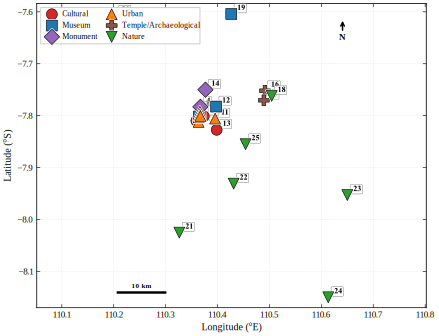
\includegraphics[width=0.95\textwidth]{fig1_attraction_map.png}
\caption{Spatial distribution of 25 tourist attractions in Yogyakarta Special Region.}
\label{fig:attraction_map}
\end{figure*}

\subsection{Algorithm Implementations}

All algorithms were implemented in Python with NumPy vectorisation. The core mechanisms are formalised below.

\textbf{ACO transition rule.} Both MMAS and ACS construct tours by having $m = 25$ ants choose the next city probabilistically. For ant $k$ at city $i$, the probability of moving to unvisited city $j$ is:
\begin{equation}
  p_{ij}^{k} = \frac{[\tau_{ij}]^{\alpha}\,[\eta_{ij}]^{\beta}}
    {\displaystyle\sum_{l \in \mathcal{N}_{i}^{k}} [\tau_{il}]^{\alpha}\,[\eta_{il}]^{\beta}},
    \quad j \in \mathcal{N}_{i}^{k}
  \label{eq:aco_prob}
\end{equation}
where $\tau_{ij}$ is the pheromone on edge $(i,j)$, $\eta_{ij} = 1/d(i,j)$ is the heuristic desirability, $\mathcal{N}_{i}^{k}$ is the set of unvisited cities, and $\alpha$, $\beta$ control the relative influence of pheromone versus distance.

\textbf{MMAS} \cite{stutzle2000} restricts pheromone trails to $[\tau_{\min}, \tau_{\max}]$. After each iteration, only the best ant deposits pheromone:
\begin{equation}
  \tau_{ij} \leftarrow \mathrm{clamp}\!\bigl[(1-\rho)\,\tau_{ij} + \Delta\tau_{ij}^{\mathrm{best}},\;\tau_{\min},\;\tau_{\max}\bigr]
  \label{eq:mmas_update}
\end{equation}
where $\Delta\tau_{ij}^{\mathrm{best}} = 1/D^{\mathrm{best}}$ if edge $(i,j)$ belongs to the best tour. Bounds are set as $\tau_{\max} = 1/(\rho \cdot D_{\mathrm{NN}})$ and $\tau_{\min} = \tau_{\max}/(2n)$. Parameters: $\alpha = 1.0$, $\beta = 3.0$, $\rho = 0.02$, 500 iterations, stagnation re-initialisation after 100 iterations without improvement.

\textbf{ACS} \cite{dorigo1997} uses a pseudo-random proportional rule: with probability $q_0$ the ant greedily selects $\arg\max_{j}[\tau_{ij}]^{\alpha}[\eta_{ij}]^{\beta}$; otherwise it samples from Eq.~\eqref{eq:aco_prob}. After each step, local pheromone decay is applied: $\tau_{ij} \leftarrow (1-\xi)\,\tau_{ij} + \xi\,\tau_0$, with $\tau_0 = 1/(n \cdot D_{\mathrm{NN}})$. Parameters: $q_0 = 0.9$, $\xi = 0.1$, $\rho = 0.1$, 500 iterations.

\textbf{GA} used Order Crossover (OX) on permutation chromosomes with population 100, crossover rate 0.8, swap mutation rate 0.02, tournament selection ($k = 3$), 10\% elitism, 500 generations with early stopping after 100 generations without improvement.

\textbf{SA} explores the neighbourhood by 2-opt moves. At temperature $T$, a candidate solution with cost difference $\Delta D = D' - D$ is accepted with probability:
\begin{equation}
  P(\text{accept}) =
  \begin{cases}
    1 & \text{if } \Delta D < 0 \\
    \exp(-\Delta D / T) & \text{otherwise}
  \end{cases}
  \label{eq:sa_accept}
\end{equation}
A 2-opt move reverses a subtour segment between positions $i$ and $j$. The cost change is evaluated in $O(1)$:
\begin{multline}
  \Delta D = d(\pi_i, \pi_j) + d(\pi_{i+1}, \pi_{j+1}) \\
           - d(\pi_i, \pi_{i+1}) - d(\pi_j, \pi_{j+1})
  \label{eq:2opt_delta}
\end{multline}
Parameters: $T_0 = 10{,}000$, cooling rate $\gamma = 0.999$, $T_{\mathrm{end}} = 1.0$, 50 iterations per temperature step (${\sim}9{,}200$ total steps).

\textbf{Nearest Neighbour (NN)} baseline was executed from all 25 starting nodes; the shortest tour was reported.

\subsection{Experimental Design}

Each stochastic algorithm was executed 30 times with seeds 42--71. The experimental programme consisted of four parts: (1)~main comparison, with 120 stochastic runs (30 per algorithm) plus one deterministic NN run; (2)~parameter sensitivity, testing 27 MMAS configurations by combining three levels each of pheromone weight (0.5, 1.0, 2.0), heuristic weight (2, 3, 5), and evaporation rate (0.02, 0.05, 0.10), with 10 runs per configuration; (3)~scalability analysis on subsets of 10, 12, 15, and 20 attractions, 10 runs each; and (4)~Wilcoxon signed-rank tests at a 0.05 significance level for all six pairwise algorithm comparisons.

\textbf{Performance metrics.} Algorithm quality is measured by the Relative Percentage Deviation (RPD) from the best-known solution $D^{*}$:
\begin{equation}
  \mathrm{RPD} = \frac{D - D^{*}}{D^{*}} \times 100\%
  \label{eq:rpd}
\end{equation}
Solution consistency is assessed by the Coefficient of Variation (CV), defined as the standard deviation divided by the mean distance. Computational efficiency is reported as mean wall-clock time per run.


%% ============================================================
\section{Results and Discussion}
\label{sec:results}
%% ============================================================

\subsection{Algorithm Performance}

Table~\ref{tab:performance} summarises all 30 independent runs per algorithm. SA and MMAS both discovered the same best-known tour of \SI{283.76}{km}, but SA was far more consistent, with a mean only \SI{0.06}{km} above the best and a standard deviation of just \SI{0.08}{km}. SA's RPD of 0.02\% and CV of 0.03\% stand in sharp contrast to GA's 6.47\% RPD and 2.25\% CV, reflecting the difference between a tightly focused local search and a population-based method that struggles with permutation structure. ACS offers a practical middle ground: its tours averaged about \SI{1.7}{km} longer than SA's, but it ran 10.7 times faster (\SI{0.327}{s} versus \SI{3.496}{s}). GA performed worst overall, with a mean tour length that exceeded even the deterministic NN baseline, confirming that basic OX crossover alone cannot solve this 25-node problem effectively.

\begin{table*}[!t]
\centering
\caption{Algorithm performance comparison over 30 independent runs. Best values in bold; NN is deterministic (single run). RPD is computed from the best-known distance $D^{*} = \SI{283.76}{km}$.}
\label{tab:performance}
\footnotesize
\begin{tabular}{@{}l
  S[table-format=3.2]
  S[table-format=3.2]
  S[table-format=3.2]
  S[table-format=1.2]
  S[table-format=1.2]
  S[table-format=1.2]
  S[table-format=1.3]@{}}
\toprule
{Algorithm} & {Best (km)} & {Mean (km)} & {Worst (km)} & {Std (km)} & {RPD (\%)} & {CV (\%)} & {Time (s)} \\
\midrule
MMAS & 283.76 & 284.35 & 286.71 & 0.85 & 0.21 & 0.30 & 1.704 \\
ACS  & 283.94 & 285.49 & 288.48 & 1.80 & 0.61 & 0.63 & \bfseries 0.327 \\
GA   & 291.31 & 302.13 & 318.03 & 6.79 & 6.47 & 2.25 & 0.676 \\
\textbf{SA} & \bfseries 283.76 & \bfseries 283.82 & \bfseries 283.97 & \bfseries 0.08 & \bfseries 0.02 & \bfseries 0.03 & 3.496 \\
NN   & {297.10} & {297.10} & {297.10} & {0.00} & {4.70} & {0.00} & {0.001} \\
\bottomrule
\end{tabular}
\end{table*}

The run-level distributions in Fig.~\ref{fig:boxplot} reveal how each algorithm explores the solution space. SA found the global optimum in 19 of 30 runs; the remaining 11 settled on one of three near-optimal tours within \SI{0.21}{km} of the best, showing that the 2-opt neighbourhood funnels solutions toward a small family of structurally similar tours. MMAS hit the optimum only once, but 19 runs still fell within 0.06\% of it, forming a tight cluster. ACS shows a distinct bimodal pattern: about half the runs reached its best tour, while the other half got trapped on longer routes because the high exploitation probability (0.9) can lock the colony onto early pheromone trails. GA produced the widest spread (\SI{26.7}{km} between best and worst), with no concentration around any single tour structure.

\begin{figure*}[!t]
\centering
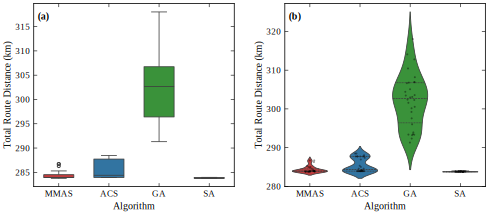
\includegraphics[width=0.95\textwidth]{fig4_boxplot.png}
\caption{Distribution of best distances across 30 runs. Box plots show median, interquartile range, and outliers; violin overlays show kernel density.}
\label{fig:boxplot}
\end{figure*}

Table~\ref{tab:wilcoxon} reports the Wilcoxon signed-rank test results for all six pairwise comparisons. Every pair is statistically significant ($p < 0.05$), establishing the ranking SA $>$ MMAS $>$ ACS $>$ GA. Even the closest pair, MMAS versus ACS, yielded $p = 0.011$, while the remaining five returned $p < 0.0001$. For every pair involving GA, all 30 matched observations favoured the competing algorithm ($W = 0$).

\begin{table*}[!t]
\centering
\caption{Wilcoxon signed-rank test results (significance level 0.05). All six pairwise comparisons are statistically significant.}
\label{tab:wilcoxon}
\footnotesize
\begin{tabular}{@{}l S[table-format=2.1] l@{\hspace{30pt}}l S[table-format=2.1] l@{}}
\toprule
{Pair} & {$W$} & {$p$-value} & {Pair} & {$W$} & {$p$-value} \\
\midrule
MMAS vs ACS & 68.0 & $0.011$     & ACS vs GA  & 0.0 & $< 0.0001$ \\
MMAS vs GA  & 0.0  & $< 0.0001$ & ACS vs SA  & 9.0 & $< 0.0001$ \\
MMAS vs SA  & 31.0 & $< 0.0001$ & GA vs SA   & 0.0 & $< 0.0001$ \\
\bottomrule
\end{tabular}
\end{table*}

\subsection{Convergence Behaviour}

Fig.~\ref{fig:convergence} plots the mean best-so-far distance over 500 iterations, averaged across 30 runs. The four algorithms converge at very different rates.

SA starts with the poorest initial solutions (random permutations), but descends the fastest and reaches its final value by roughly iteration~223, less than half the allocated budget. The 2-opt neighbourhood produces large improving moves early on, and the Metropolis criterion (Eq.~\ref{eq:sa_accept}) keeps enough randomness to escape local optima before the temperature drops too low.

MMAS follows a steadier trajectory. Its bounded pheromone trails prevent premature convergence, so the colony keeps improving until around iteration~357. The trade-off is slower final refinement compared to SA, but no run stagnated early.

ACS shows the fastest initial descent among the ACO variants, cutting over \SI{15}{km} in the first 50 iterations. It then plateaus around iteration~178, much sooner than MMAS. The high exploitation probability (0.9) drives aggressive early search but leaves too little diversity for later refinement.

GA converged the most slowly. Its initial solutions were substantially longer because it starts from purely random permutations without a nearest-neighbour seed. GA was still improving at iteration~500, suggesting the budget was insufficient and that hybridisation with local search operators could narrow the gap.

\begin{figure*}[!t]
\centering
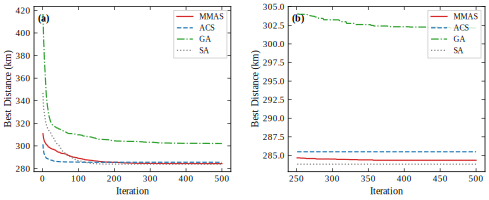
\includegraphics[width=0.95\textwidth]{fig3_convergence.png}
\caption{Convergence curves showing mean best-so-far distance over iterations (averaged across 30 runs). SA converges fastest to the lowest value; GA is still improving at iteration~500.}
\label{fig:convergence}
\end{figure*}

\subsection{Optimised Routes}

Fig.~\ref{fig:routes} compares the best routes found by each algorithm. The optimal tour (\SI{283.76}{km}, found by both SA and MMAS) traces a loop that avoids crossing legs. Starting from the urban core (Kraton, Taman Sari, Alun-Alun Kidul), the route heads southeast through Purawisata and Gembira Loka Zoo to Kotagede, then swings south to the coast (Parangtritis, Indrayanti, Goa Pindul). From there it climbs northeast through the hills (Hutan Pinus Mangunan, HeHa Sky View) to the eastern temples (Ratu Boko, Tebing Breksi, Prambanan), north to Ullen Sentalu, west to Borobudur, and back through northern Yogyakarta (Monumen Jogja Kembali, Museum Affandi, Tugu, Malioboro) to close the loop. This geographic clustering minimises backtracking across the region's distinct tourism zones.

The ACS route (Fig.~\ref{fig:routes}c) followed a nearly identical sequence, differing by only one swap in the urban core and adding less than \SI{0.2}{km}. GA's best tour (Fig.~\ref{fig:routes}d) contained visible detours where the route jumped between non-adjacent zones instead of completing one cluster before moving to the next. This is a typical weakness of OX crossover, which preserves relative ordering but does not directly optimise edge connections.

\begin{figure*}[!t]
\centering
\subfloat[SA: \SI{283.76}{km}]{\includegraphics[width=0.48\textwidth]{fig2_best_route_SA.png}}
\hfill
\subfloat[MMAS: \SI{283.76}{km}]{\includegraphics[width=0.48\textwidth]{fig2_best_route_MMAS.png}}

\vspace{4pt}

\subfloat[ACS: \SI{283.94}{km}]{\includegraphics[width=0.48\textwidth]{fig2_best_route_ACS.png}}
\hfill
\subfloat[GA: \SI{291.31}{km}]{\includegraphics[width=0.48\textwidth]{fig2_best_route_GA.png}}
\caption{Best routes found by each algorithm on the road network. Green marker: start; red: end; blue: intermediate stops. SA and MMAS share the same optimal tour structure; GA shows visible detours between geographic clusters.}
\label{fig:routes}
\end{figure*}

\subsection{Parameter Sensitivity}

Fig.~\ref{fig:sensitivity} shows how MMAS performance varies across 27 configurations (10 runs each), combining three levels each of pheromone weight, heuristic weight, and evaporation rate. The best configuration (pheromone weight 2.0, heuristic weight 2, evaporation rate 0.02) achieved a mean distance of \SI{283.82}{km}, matching SA in Table~\ref{tab:performance}, while the worst reached \SI{290.22}{km}, a \SI{6.4}{km} gap from parameter choice alone.

The interaction between pheromone weight and evaporation rate dominated. When pheromone weight is high, low evaporation works best because the colony can steadily reinforce good edges over many iterations. When pheromone weight is low, the trails carry less information and need faster refreshing; higher evaporation compensates by clearing outdated pheromone and encouraging re-exploration. At the lowest pheromone weight, raising the evaporation rate from 0.02 to 0.10 reduced the mean distance by \SI{2.3}{km}.

The heuristic weight had a smaller effect. Changing it from 2 to 5 within any panel rarely shifted the mean distance by more than \SI{1}{km}. One exception occurred at moderate pheromone weight with high heuristic weight and mid-range evaporation, where all 10 runs converged to the same tour with zero variance, a sign that a strong distance heuristic can force complete convergence at the cost of solution diversity.

\begin{figure*}[!t]
\centering
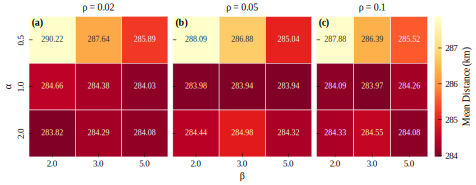
\includegraphics[width=0.95\textwidth]{fig5_parameter_sensitivity.png}
\caption{MMAS parameter sensitivity heatmaps. Each cell shows the mean distance (km) over 10 runs for a given heuristic weight and evaporation rate combination at three levels of pheromone weight. The best configuration (pheromone weight 2.0, heuristic weight 2, evaporation rate 0.02) matches SA's mean of \SI{283.82}{km}.}
\label{fig:sensitivity}
\end{figure*}

\subsection{Scalability}

Fig.~\ref{fig:scalability} reports mean distance and computation time for subsets of 10, 12, 15, and 20 attractions (10 runs each), alongside the full 25-attraction results from Table~\ref{tab:performance}. At 12 or fewer attractions, all four metaheuristics found the optimal tour in every run, though GA already showed non-zero variance at 12 attractions.

The algorithms separated at 15 attractions. MMAS, ACS, and SA still found the optimum reliably, but GA's mean rose to 3.1\% above the best-known solution. At 20 attractions, SA still produced near-perfect results, MMAS and ACS stayed within 0.2\%, but GA's gap grew to 5.2\%. This widening continued at 25 attractions, where GA trailed by 6.5\% (Table~\ref{tab:performance}).

The bottom panel of Fig.~\ref{fig:scalability} shows runtime. MMAS and ACS grew roughly quadratically with problem size, consistent with their pheromone update mechanism. GA scaled linearly. SA's runtime stayed nearly constant at about \SI{3.5}{s} regardless of problem size, since the cooling schedule, not the number of cities, governs its computation.

\begin{figure*}[!t]
\centering
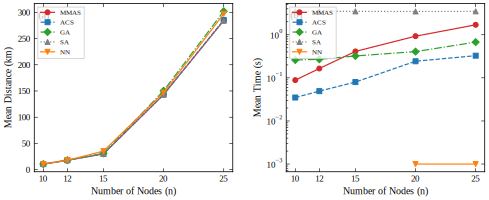
\includegraphics[width=0.95\textwidth]{fig8_scalability.png}
\caption{Scalability analysis for 10, 12, 15, 20, and 25 attractions. Top: mean distance; bottom: mean computation time. GA diverges from the other algorithms as problem size increases; SA runtime remains constant.}
\label{fig:scalability}
\end{figure*}

\subsection{Euclidean Versus Road Distance}

Euclidean distances are an imperfect proxy for actual travel. To quantify the gap, we computed the detour ratio for each attraction pair:
\begin{equation}
  r_{ij} = \frac{d_{\mathrm{road}}(i,j)}{d_{\mathrm{euclid}}(i,j)}
  \label{eq:detour_ratio}
\end{equation}
where a ratio of 1 would mean a perfectly straight road.

Fig.~\ref{fig:euclidean_road} compares the two distance measures across all 300 attraction pairs. The scatter plot shows a strong linear correlation (R-squared = 0.97), but with a consistent positive bias: road distances averaged 18\% longer (mean ratio 1.18, standard deviation 0.12). The ratio was lowest (around 1.05) for pairs connected by direct highway segments, such as the Yogyakarta--Prambanan corridor, and highest (up to 1.72) for pairs separated by rivers, mountain slopes, or dense urban fabric. Because the bias is consistent, the errors compound across a multi-stop tour. For the 25-attraction problem, relying on Euclidean distances would underestimate total tour length by roughly \SI{40}{--}\SI{50}{km}, enough to make a planned day trip infeasible.

\begin{figure*}[!t]
\centering
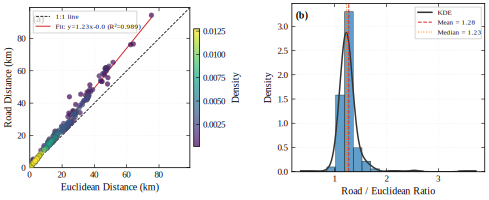
\includegraphics[width=0.95\textwidth]{fig7_euclidean_vs_road.png}
\caption{Euclidean versus road distance comparison. Left: scatter plot with linear regression (R-squared = 0.97); right: histogram of detour ratios (mean 1.18, range 1.05--1.72).}
\label{fig:euclidean_road}
\end{figure*}

\subsection{Discussion}

\textbf{Algorithm selection trade-offs.} SA with 2-opt is the best choice when a few seconds of computation is acceptable, such as offline trip planning tools or pre-computed itinerary brochures. ACS suits interactive applications better, for example a mobile app recalculating routes in real time, because it runs an order of magnitude faster while producing tours only marginally longer (Table~\ref{tab:performance}). MMAS falls between the two: more reliable than ACS ($p = 0.011$, Table~\ref{tab:wilcoxon}), but slower. GA with basic OX crossover is not competitive at this problem size (Fig.~\ref{fig:scalability}), though hybridising it with local search \cite{ruan2024} or edge-assembly crossover \cite{deng2021} would likely help.

\textbf{Practical implications.} The optimal \SI{283.76}{km} tour reported in Table~\ref{tab:performance} translates to roughly 7 hours of driving at Yogyakarta's typical mixed-road speed of \SI{40}{km/h}. Combined with 30--60 minutes spent at each attraction, visiting all 25 sites listed in Table~\ref{tab:attractions} would span 3--4 days. The geographic clustering visible in the optimal route (Fig.~\ref{fig:routes}a) suggests a natural breakdown into daily itineraries: (1)~the urban core (Kraton, Malioboro, Taman Sari, and surrounding sites), (2)~the eastern temple complex (Prambanan, Ratu Boko, Tebing Breksi) combined with the northern highland (Ullen Sentalu), (3)~the southern coast (Parangtritis, Indrayanti, Goa Pindul, Hutan Pinus), and (4)~a western excursion to Borobudur. Tour operators could use these clusters as ready-made day-trip modules.

\textbf{Comparison with related work.} The 18\% road-to-Euclidean deviation matches findings by Boyaci et al. \cite{boyaci2021} for European vehicle routing and Tatit et al. \cite{tatit2024} for spatial query accuracy, indicating that this bias is not specific to Yogyakarta. Unlike Sun et al. \cite{sun2022} and Nasution et al. \cite{nasution2024}, who used simplified distance metrics, our results show that real road distances alter both absolute tour lengths and the relative ranking of near-optimal solutions. The parameter sensitivity results also align with the tuning guidance of Kaushik and Nadeem \cite{kaushik2024}, who noted that ACO parameters interact and should not be tuned in isolation.

\textbf{Limitations.} This study optimises total distance only. Travellers also care about travel time, entrance fees, opening hours, and personal preferences; multi-objective formulations \cite{ruizmeza2022,sun2022} would address these. The road distances are static and do not account for traffic congestion or time-of-day variations. The analysis covers a single destination with 25 attractions; testing on larger instances or other Indonesian cities would test generalisability. Orienteering formulations with time windows \cite{sylejmani2024,fathurrohman2025} and near-exact solvers such as LKH \cite{zheng2023} were not included and are natural extensions.


%% ============================================================
\section{Conclusion}
\label{sec:conclusion}
%% ============================================================

This study compared four metaheuristic algorithms (MMAS, ACS, GA, and SA) for a 25-attraction tourism route optimisation problem in Yogyakarta, formulated as a TSP over real road distances extracted from OpenStreetMap. Three principal findings emerged. First, SA with 2-opt consistently produced the shortest and most reliable tours, achieving a mean of \SI{283.82}{km} across 30 runs with a standard deviation below \SI{0.1}{km}. All pairwise differences were statistically significant (p < 0.05), yielding a clear ranking of SA, MMAS, ACS, and GA from best to worst. Second, ACS offered the best speed--quality trade-off, completing runs an order of magnitude faster than SA while producing tours only marginally longer, making it suitable for real-time applications. Third, the mean road-to-Euclidean detour ratio of 1.18 confirms that Euclidean distances systematically underestimate travel costs, reinforcing the need for real road network data in tourism route planning.

Parameter sensitivity analysis revealed that MMAS performance varies by up to \SI{6.4}{km} depending on parameter settings, with a strong interaction between the pheromone weight and evaporation rate. Scalability tests showed that GA's quality gap widens with problem size, while the other three algorithms remain robust up to 25 attractions.

Future work should extend this framework to multi-objective formulations that include travel time, visitor preferences, and time-window constraints, and should incorporate dynamic traffic data. Testing the approach on other Indonesian tourism destinations would help assess generalisability.


%% ============================================================
%% Back matter
%% ============================================================
\section*{Declaration of Competing Interest}
The authors declare no known competing financial interests or personal relationships that could have influenced this work.

\section*{Data Availability}
The source code, distance matrices, and experimental results are available at [repository URL].

\bibliographystyle{IEEEtran}
\bibliography{references}

\end{document}
